% Copyright 2004 by Till Tantau <tantau@users.sourceforge.net>.
%
% In principle, this file can be redistributed and/or modified under
% the terms of the GNU Public License, version 2.
%
% However, this file is supposed to be a template to be modified
% for your own needs. For this reason, if you use this file as a
% template and not specifically distribute it as part of a another
% package/program, I grant the extra permission to freely copy and
% modify this file as you see fit and even to delete this copyright
% notice. 

\documentclass[handout]{beamer}
% Replace the \documentclass declaration above
% with the following two lines to typeset your 
% lecture notes as a handout:
%\documentclass{article}
\usepackage{CJKutf8}
\usepackage[T1]{fontenc}
%\usepackage[utf8x]{inputenc}
\usepackage{graphicx}
\usepackage{ulem}
\usepackage{url}

% There are many different themes available for Beamer. A comprehensive
% list with examples is given here:
% http://deic.uab.es/~iblanes/beamer_gallery/index_by_theme.html
% You can uncomment the themes below if you would like to use a different
% one:
%\usetheme{AnnArbor}
%\usetheme{Antibes}
%\usetheme{Bergen}
%\usetheme{Berkeley}
%\usetheme{Berlin}
%\usetheme{Boadilla}
%\usetheme{boxes}
%\usetheme{CambridgeUS}
%\usetheme{Copenhagen}
%\usetheme{Darmstadt}
%\usetheme{default}
%\usetheme{Frankfurt}
\usetheme{Goettingen}
%\usetheme{Hannover}
%\usetheme{Ilmenau}
%\usetheme{JuanLesPins}
%\usetheme{Luebeck}
%\usetheme{Madrid}
%\usetheme{Malmoe}
%\usetheme{Marburg}
%\usetheme{Montpellier}
%\usetheme{PaloAlto}
%\usetheme{Pittsburgh}
%\usetheme{Rochester}
%\usetheme{Singapore}
%\usetheme{Szeged}
%\usetheme{Warsaw}

\begin{document}
\begin{CJK}{UTF8}{gbsn}

\title{内存体系结构}

% A subtitle is optional and this may be deleted
\subtitle{原理与应用}

\author{李庚\inst{1}}
% - Give the names in the same order as the appear in the paper.
% - Use the \inst{?} command only if the authors have different
%   affiliation.

\institute[Qunar.com] % (optional, but mostly needed)
{
  \inst{1}%
  旅游度假SI \\
  新业务部
}
% - Use the \inst command only if there are several affiliations.
% - Keep it simple, no one is interested in your street address.

\date{Apr. 28th, 2014}
% - Either use conference name or its abbreviation.
% - Not really informative to the audience, more for people (including
%   yourself) who are reading the slides online

\subject{2014技术分享}
% This is only inserted into the PDF information catalog. Can be left
% out. 

% If you have a file called "university-logo-filename.xxx", where xxx
% is a graphic format that can be processed by latex or pdflatex,
% resp., then you can add a logo as follows:

% \pgfdeclareimage[height=0.5cm]{university-logo}{university-logo-filename}
% \logo{\pgfuseimage{university-logo}}

% Delete this, if you do not want the table of contents to pop up at
% the beginning of each subsection:
\AtBeginSubsection[]
{
  \begin{frame}<beamer>{纲要}
    \tableofcontents[currentsection,currentsubsection]
  \end{frame}
}

% Let's get started

\begin{frame}
  \titlepage
\end{frame}

\begin{frame}{纲要}
  \tableofcontents
  % You might wish to add the option [pausesections]
\end{frame}

% Section and subsections will appear in the presentation overview
% and table of contents.
\section{Programmer眼中的内存是什么?}

\subsection{Coding角度}
\begin{frame}{程序能够处理的数据的存储源}
  \begin{itemize}
  \item {
      int a = 10; Date date = new Date("2014-06-28");
      Arrays.sort(...);
      \pause
  }
  \item {
      不在内存中的数据必须通过IO操作读入内存后才能使用
  }
  \end{itemize}
\end{frame}

\subsection{系统资源角度}
\begin{frame}{访问性能较好的稀缺资源}
  \begin{itemize}
  \item {
      OutOfMemoryException
      \pause
  }
  \item {
      check\_swap warning: 程序性能恶化的标识之一
      \pause
  }
  \item {
      合理使用内存是保证程序质量的重要前提
  }
  \end{itemize}
\end{frame}

\section{Memory Access Basics}

\subsection{基本流程}

\begin{frame}{一个简单的例子 (C)}
  \begin{itemize}
  \item {
      long a = 35; \\
      long* p = \&a; \\
      long pa = (long)p; \\
      \pause
      printf("0x\%lx", pa); // 0x7fff50f18638 \\
      \pause
      printf("\%ld", *((long*)pa)); // 35
      \pause
  }
  \item {
      内存地址:可以用来获取数据的数据
  }
  \item {
      不同体系结构下,地址的长度不同
  }
  \end{itemize}
\end{frame}

\begin{frame}{基本流程}
  \begin{block}{程序使用的地址为虚拟地址(Virtual Address)}
    \begin{itemize}
      \item {
          printf("0x\%lx", pa); // 0x7fff50f18638 \\
          printf("\%ld", *((long*)pa)); // 35
      }
    \end{itemize}
  \end{block}
  \begin{block}{硬件+操作系统进行分页管理}
    \begin{itemize}
      \item {
          硬件负责:Virtual Address -> MMU -> Physical Address -> Data
          \begin{center}
            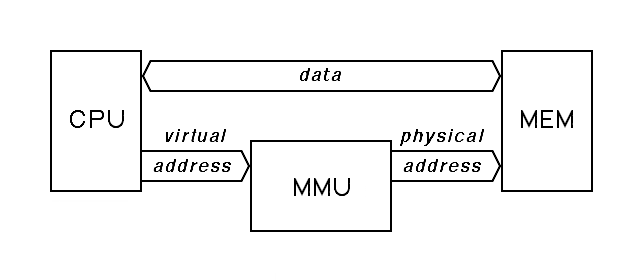
\includegraphics[scale=0.3]{./images/cpu-mmu}
          \end{center}
      }
    \end{itemize}
  \end{block}
\end{frame}

\begin{frame}{基本流程}
  \begin{block}{}
    \begin{itemize}
      \item {
          操作系统负责:每个进程的Page Table设置
      }
    \end{itemize}
    \begin{center}
      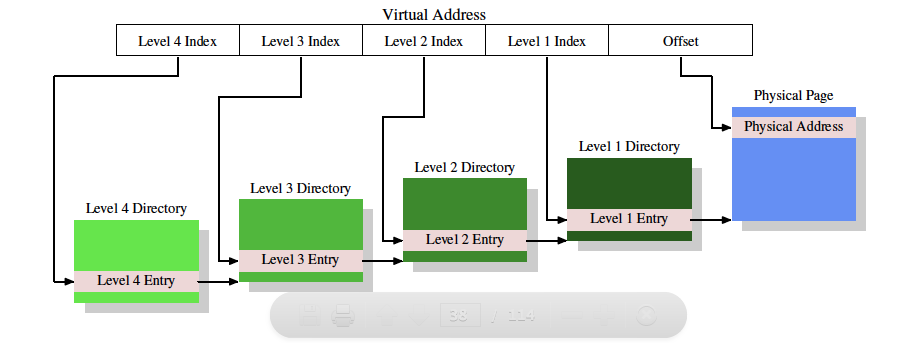
\includegraphics[scale=0.22]{./images/page-table}
    \end{center}
  \end{block}
\end{frame}

\subsection{访问性能上的考虑}

\begin{frame}{要点:如何使CPU尽快取到需要的数据?}
  \begin{block}{程序的局部性原理(Locality)}
    \begin{itemize}
      \item {
          for (int i = 0; i < myArray.length; ++i) { \\
            myArray[i] += c; \\
          }
          \pause
      }
      \item {
          时间局部性(Temporal Locality):被访问过的数据短时间内很可能再次被使用。
      }
      \item {
          空间局部性(Spatial Locality):与被访问的数据空间上相邻的数据很可能在最近的将来被访问。
      }
    \end{itemize}
  \end{block}
\end{frame}

\begin{frame}{CPU Cache}
  \begin{block}{存在于CPU和内存之间的一层数据存储}
    \begin{center}
      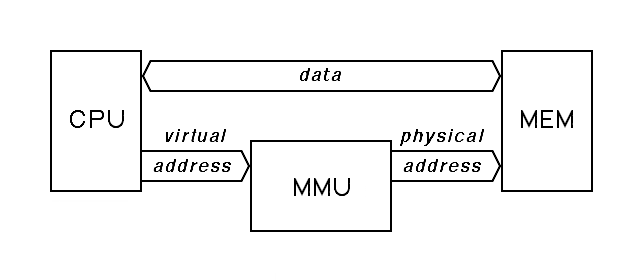
\includegraphics[scale=0.2]{./images/cpu-mmu}
      \pause
      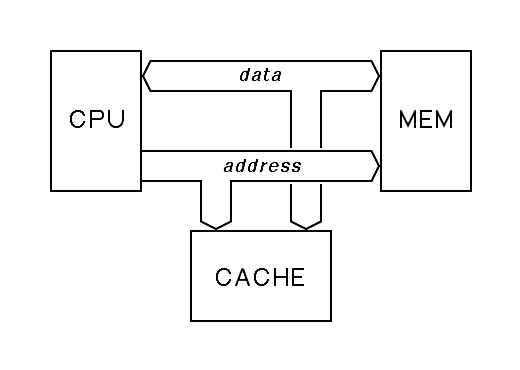
\includegraphics[scale=0.2]{./images/cpu-cache-memory}
    \end{center}
  \end{block}
\end{frame}

\begin{frame}{Cache的特性}
  \begin{block}{容量较小}
    \begin{itemize}
      \item {
          容量在kB - mB数量级
      }
    \end{itemize}
  \end{block}  
  \begin{block}{访问速度快}
    \begin{itemize}
      \item {
          L1 cache reference: 0.5ns \\
          L2 cache reference: 7ns \\
          Main memory reference: 100ns \\
          (Jeff Dean, Numbers everyone should know)
      }
    \end{itemize}
  \end{block}
  \begin{block}{美丽的愿景}
    \begin{itemize}
      \item {
          所有内存访问都能够在Cache中命中
      }
    \end{itemize}
  \end{block}
\end{frame}

\begin{frame}{程序开发人员能做什么}
  \begin{block}{示例:计算二维平面上N个点的內积(inner product)}
    \pause
    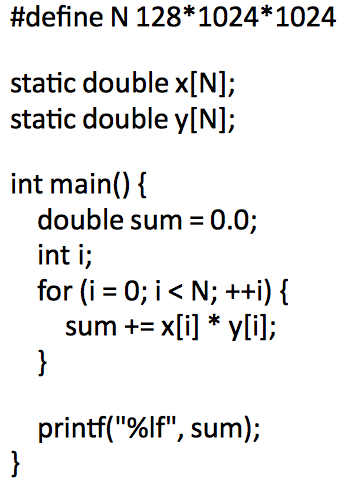
\includegraphics[scale=0.3]{./images/inner-product-miss}
    \pause
    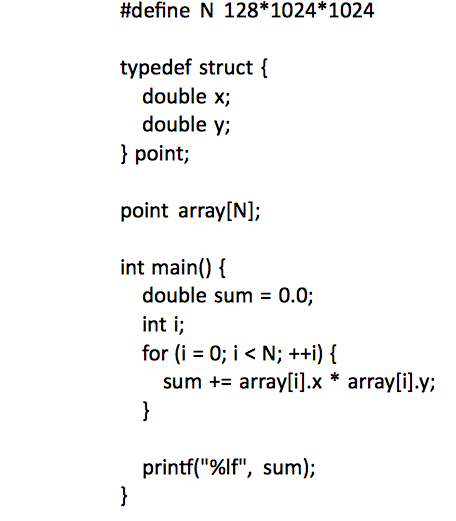
\includegraphics[scale=0.3]{./images/inner-product-hit}
    \pause
  \end{block}
  \begin{block}{原则1:尽可能顺序访问,充分利用空间局部性}
  \end{block}
\end{frame}

\begin{frame}{分页机制带来的挑战}
  \begin{block}{}
    \begin{center}
      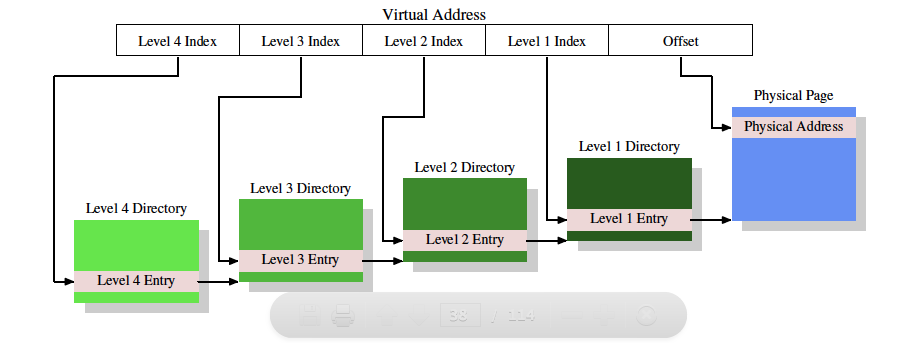
\includegraphics[scale=0.22]{./images/page-table}
    \end{center}
    \pause
  \end{block}
  \begin{block}{每次虚拟地址到物理地址转换需要访问内存的次数}
    \begin{itemize}
      \item {Page Directory在内存中,每级Directory访问对应一次内存访问 \pause}
      \item {每级Page Directory的访问依赖于前一级的访问结果,无法通过cpu的流水线优化 \pause}
      \item {即使每级访问CPU的data cache都命中,需要的CPU时钟周期与页目录级数成线性关系}
    \end{itemize}
  \end{block}
\end{frame}

\begin{frame}{分页机制带来的挑战(续)}
  \begin{block}{}
    \begin{center}
      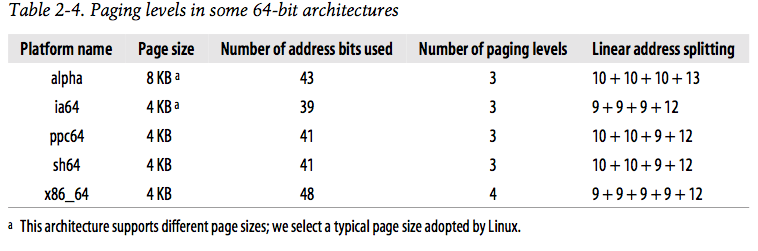
\includegraphics[scale=0.3]{./images/page-table-levels}
    \end{center}
    \pause
  \end{block}
  \begin{block}{地址映射的过程可能比数据访问本身还要慢}
  \end{block}
\end{frame}

\begin{frame}{TLB: Translation Look-aside Buffer}
  \begin{block}{直接将虚拟地址向物理地址的映射结果缓存起来}
    \begin{itemize}
      \item {名为Buffer,实为Cache}
      \item {TLB不命中时,通过页表进行映射}
    \end{itemize}    
  \end{block}
  \begin{block}{}
    \begin{center}
      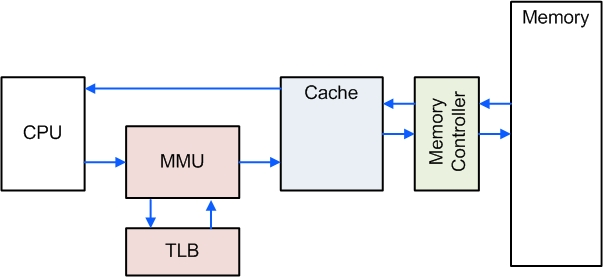
\includegraphics[scale=0.4]{./images/mmu-tlb}
    \end{center}
  \end{block}
\end{frame}

\begin{frame}{如何避免TLB Miss}
  \begin{block}{原则2:即使Cache能够容纳足够多的数据,也要尽量将与计算无关的数据剥离。}
    \begin{itemize}
      \item {缩小虚拟地址空间范围降低Miss的概率}
      \item {
          typedef struct \{ \\
            double x; \\
            double y; \\
            \sout{char data[128];} \\
          \} point;
        }
    \end{itemize}
  \end{block}
\end{frame}

\section{硬件上Cache效率的优化}

\begin{frame}{提升Cache访问效率的常用方法}
  \begin{itemize}
    \item {i-cache与d-cache分离}
    \item {增大容量,调整关联度}
    \item {Aligned Access}
    \item {Hardware Prefetch}
  \end{itemize}
\end{frame}

\begin{frame}{Cache应该缓存虚拟地址 vs. 物理地址?}
  \begin{block}{}
    \begin{center}
      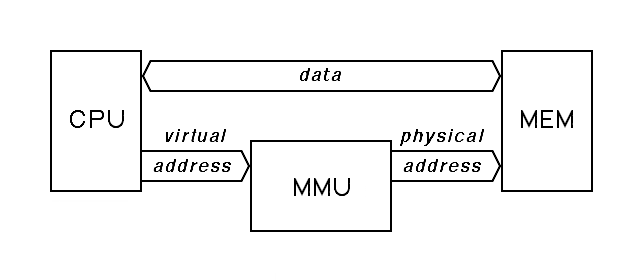
\includegraphics[scale=0.2]{./images/cpu-mmu}
      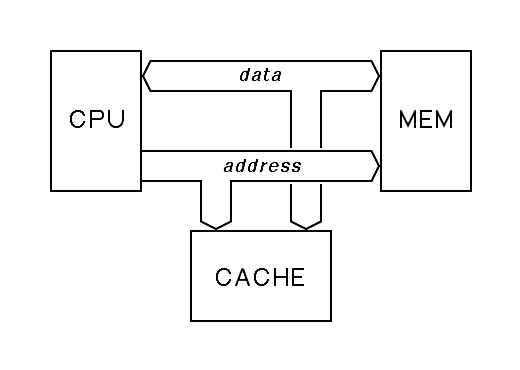
\includegraphics[scale=0.2]{./images/cpu-cache-memory}
    \end{center}
    \pause
  \end{block}
  \begin{block}{虚拟地址 vs. 物理地址}
    \begin{itemize}
      \item {不同线程的虚拟地址会冲突,线程切换的时候要清空Cache,而物理地址没有这个问题; \pause}
      \item {但是,物理地址需要虚拟地址经过MMU转换得到,可能比较慢; \pause}
    \end{itemize}
  \end{block}
\end{frame}

\begin{frame}{虚拟地址 vs. 物理地址?}
  \begin{block}{低级别(L1)用虚拟地址,高级别用物理地址}
    \begin{itemize}
      \item{低级别Cache容量小,清空的代价相对低;\pause}
      \item {用虚拟地址访问低级别Cache的同时走MMU转换,可以隐藏一部分访问延时}
    \end{itemize}
  \end{block}
\end{frame}
% \subsection{Second Subsection}

% You can reveal the parts of a slide one at a time
% with the \pause command:
%% \begin{frame}{Second Slide Title}
%%   \begin{itemize}
%%   \item {
%%     First item.
%%     \pause % The slide will pause after showing the first item
%%   }
%%   \item {   
%%     Second item.
%%   }
%%   % You can also specify when the content should appear
%%   % by using <n->:
%%   \item<3-> {
%%     Third item.
%%   }
%%   \item<4-> {
%%     Fourth item.
%%   }
%%   % or you can use the \uncover command to reveal general
%%   % content (not just \items):
%%   \item<5-> {
%%     Fifth item. \uncover<6->{Extra text in the fifth item.}
%%   }
%%   \end{itemize}
%% \end{frame}


% Placing a * after \section means it will not show in the
% outline or table of contents.
\section*{总结}

\begin{frame}{总结}
  \begin{block}{RAM访问基本过程}
    \begin{itemize}
      \item {虚拟地址通过MMU转换成物理地址,进而到物理内存中获取数据}
      \item {Cache, TLB在这个过程中的作用}
    \end{itemize}    
  \end{block}
  \begin{block}{开发过程中需要掌握的原则}
  \begin{itemize}
    \item {原则1:尽可能顺序访问,充分利用空间局部性}
    \item {原则2:即使Cache能够容纳足够多的数据,也要尽量将与计算无关的数据剥离。}
  \end{itemize}
  \end{block}
\end{frame}

\appendix
\section<presentation>*{\appendixname}
\subsection<presentation>*{推荐阅读}

\begin{frame}
  \frametitle<presentation>{推荐阅读}
    
  \begin{thebibliography}{10}
    
  \beamertemplatearticlebibitems
  % Followed by interesting articles. Keep the list short. 

  \bibitem{drepper}
    Ulrich Drepper
    \newblock {What Every Programmer Should Know About Memory}
    \newblock {\url{http://www.akkadia.org/drepper/cpumemory.pdf}}

  \bibitem{ulk}
    Daniel P. Bovet, Marco Cesati
    \newblock {Understanding the Linux Kernel, 3rd Edition, Chapter Two - Memory Addressing}
  \end{thebibliography}

  \beamertemplate
\end{frame}


% All of the following is optional and typically not needed. 
%% \appendix
%% \section<presentation>*{\appendixname}
%% \subsection<presentation>*{For Further Reading}

%% \begin{frame}[allowframebreaks]
%%   \frametitle<presentation>{For Further Reading}
    
%%   \begin{thebibliography}{10}
    
%%   \beamertemplatebookbibitems
%%   % Start with overview books.

%%   \bibitem{Author1990}
%%     A.~Author.
%%     \newblock {\em Handbook of Everything}.
%%     \newblock Some Press, 1990.
 
    
%%   \beamertemplatearticlebibitems
%%   % Followed by interesting articles. Keep the list short. 

%%   \bibitem{Someone2000}
%%     S.~Someone.
%%     \newblock On this and that.
%%     \newblock {\em Journal of This and That}, 2(1):50--100,
%%     2000.
%%   \end{thebibliography}
%% \end{frame}

\clearpage
\end{CJK}
\end{document}
